% % % %
% % % % Overview
% % % %
\section{Overview} 

\subsection{Competition Details}
\begin{frame}\frametitle{Data} 
\par \textbf{Goal}: Identify signs of diabetic retinopathy in eye images
\par \textbf{Given}: 35126 images for training, 53576 images in test set
\par Images are big: 2500x2000 and larger
\par Compressed data size: 88Gb

\vspace{5pt}

\begin{tabular}{|@{}c@{}|@{}c@{}|@{}c@{}|@{}c@{}|@{}c@{}|}
\hline
	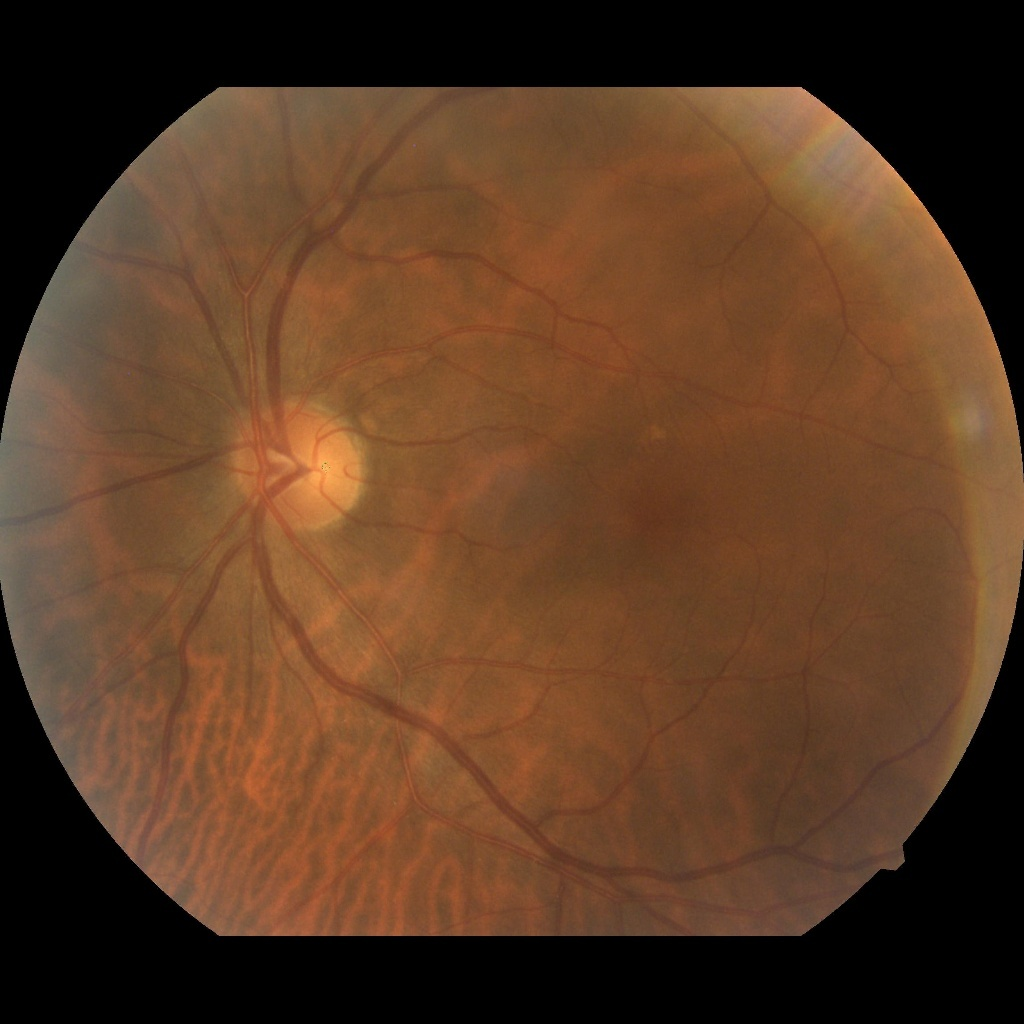
\includegraphics[width=0.2\textwidth]{pics/classified_samples/197_left_0.jpg} &
	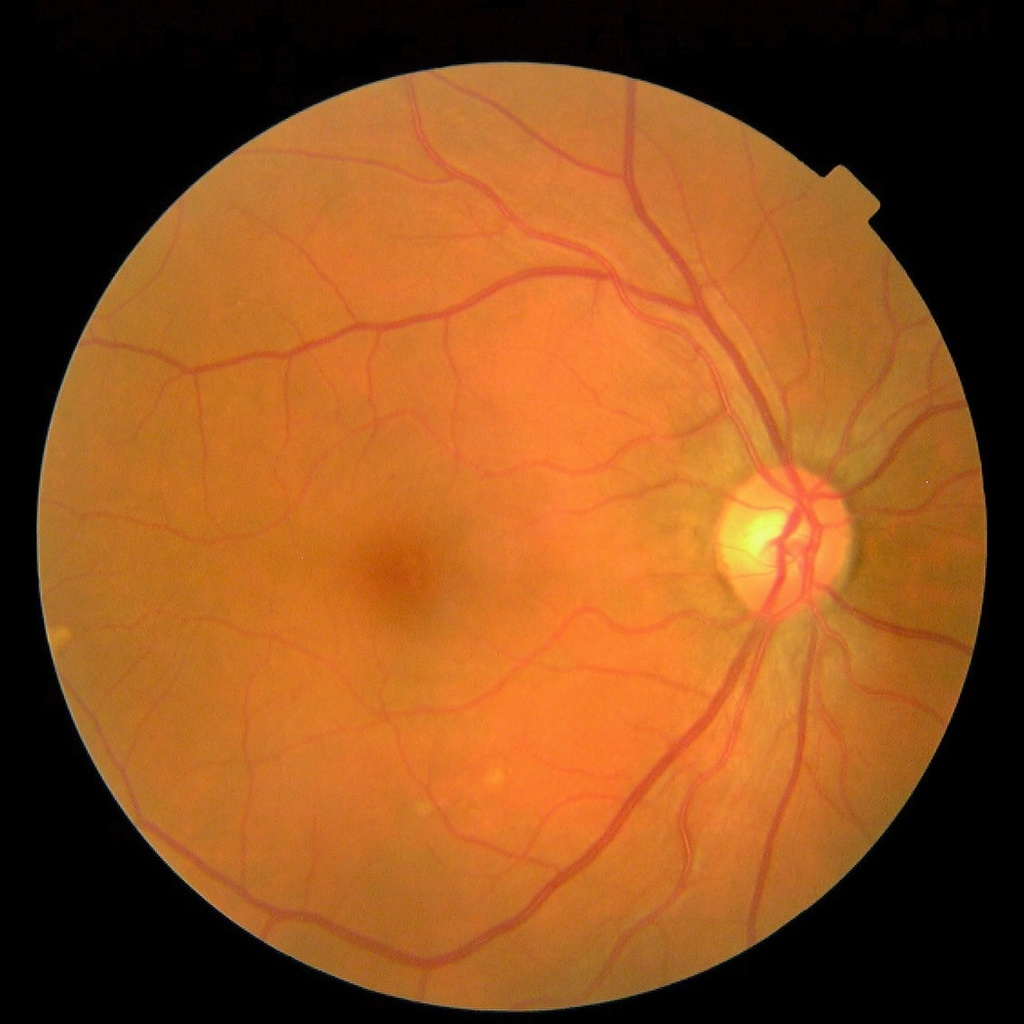
\includegraphics[width=0.2\textwidth]{pics/classified_samples/204_right_1.jpg} &
	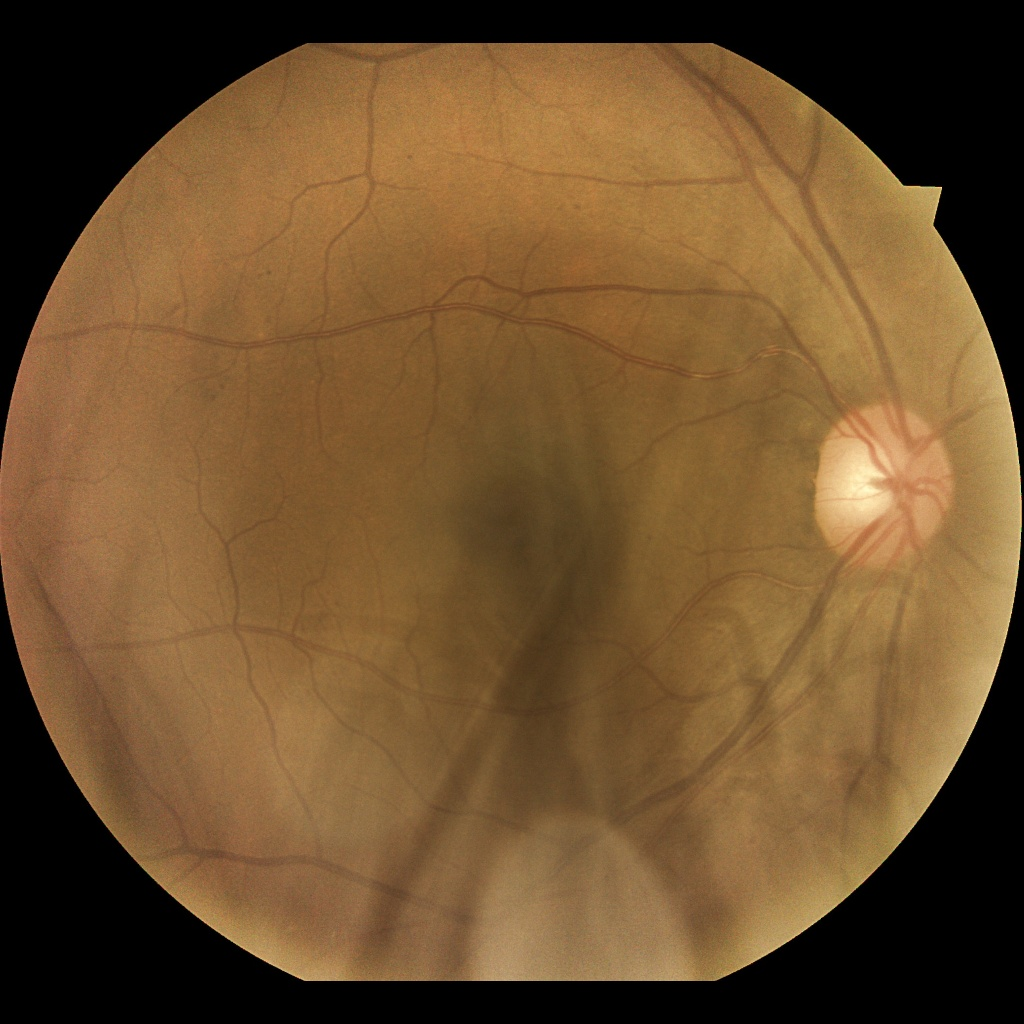
\includegraphics[width=0.2\textwidth]{pics/classified_samples/82_right_2.jpg} &
	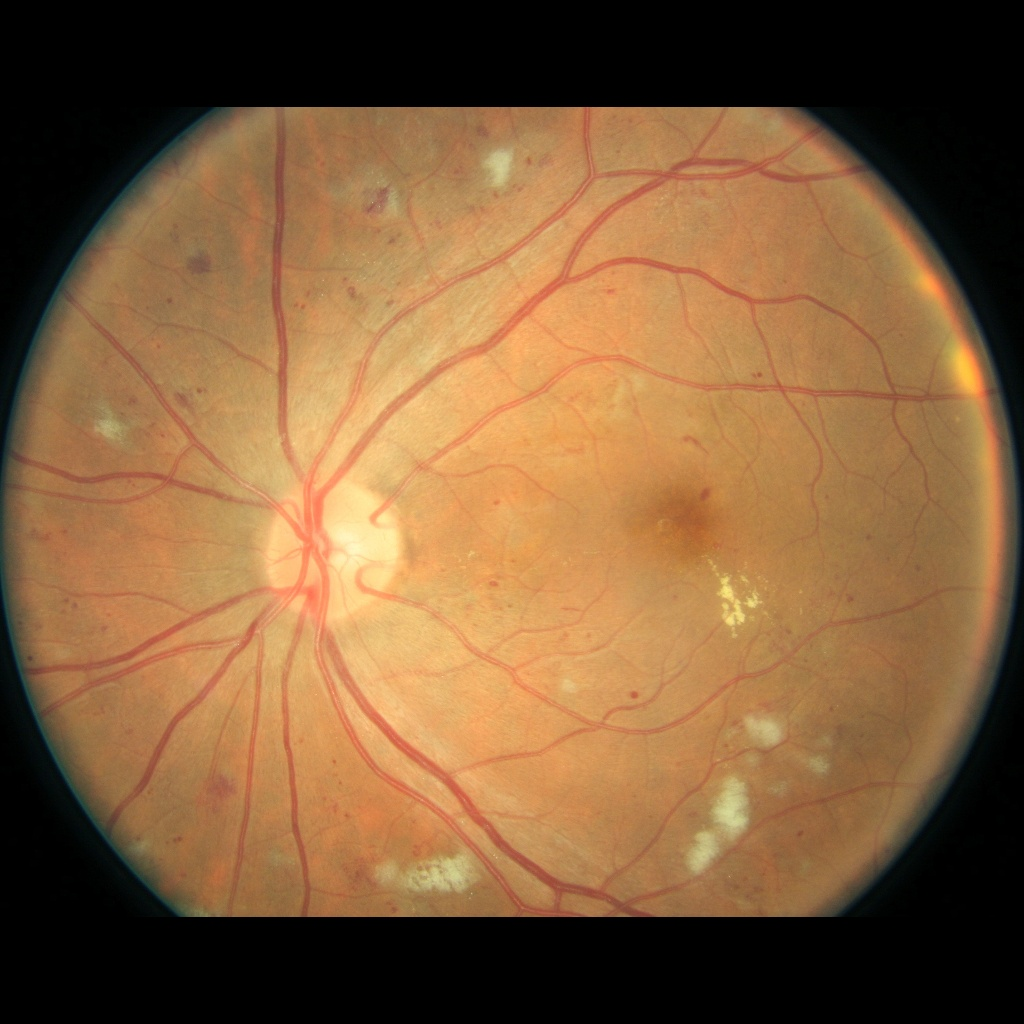
\includegraphics[width=0.2\textwidth]{pics/classified_samples/687_right_3.jpg} &
	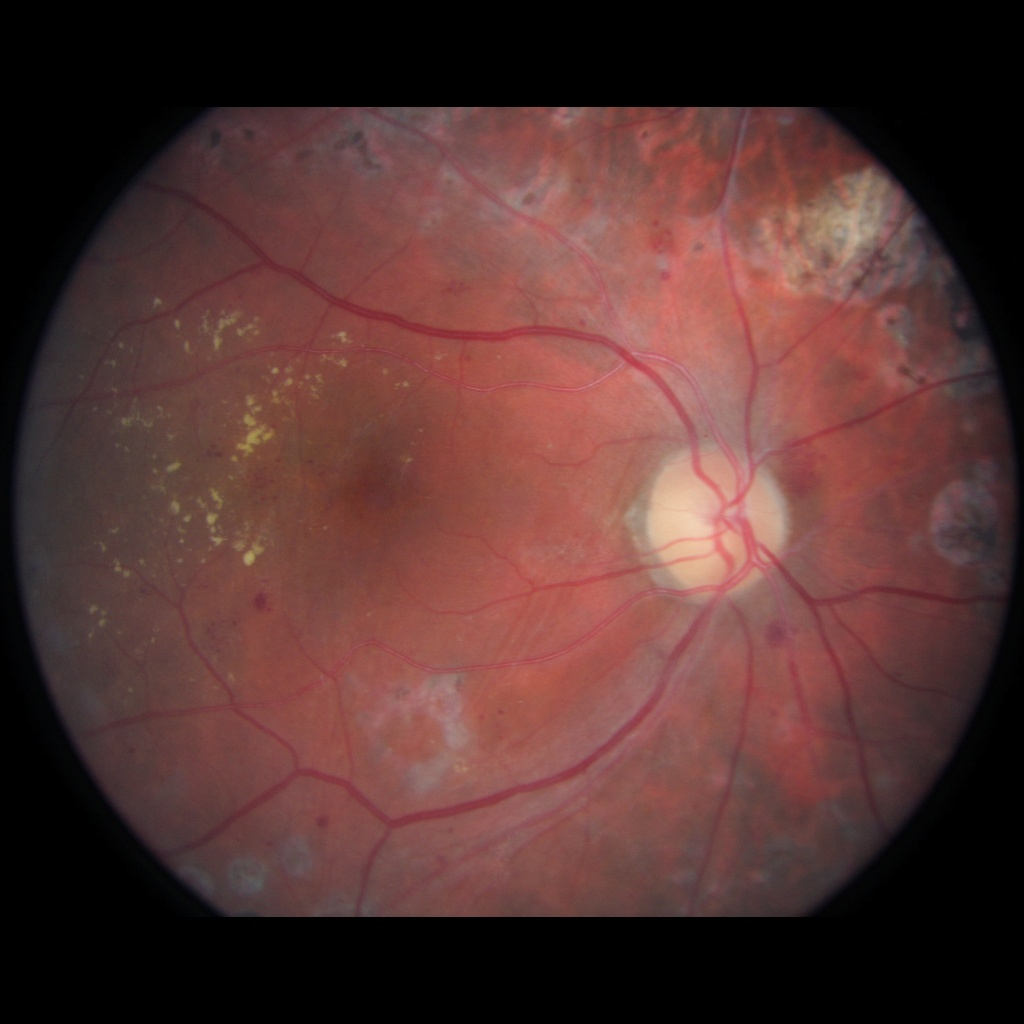
\includegraphics[width=0.2\textwidth]{pics/classified_samples/2496_left_4.jpg} \\\noalign{\vspace{-0.15cm}}
\hline

Normal & Mild & Moderate & Severe & Proliferative \\

\hline
 \specialcell{25810\\ \footnotesize{73.48\%}}  & 
 \specialcell{2443\\\footnotesize6.96\%} & 
 \specialcell{5292\\\footnotesize15.07\%} & 
 \specialcell{873\\\footnotesize2.48\%} & 
 \specialcell{708\\\footnotesize2.01\%} \\

\hline
\end{tabular}

\end{frame}

\begin{frame}\frametitle{Quality metric I: Cohen's kappa}
\footnotesize
Cohen's kappa measures the agreement between two raters who each classify $N$ items into $C$ mutually exclusive categories. 



\[ \kappa = \frac{p_o - p_e}{1 - p_e} = 1- \frac{1 - p_o}{1 - p_e}, \]

where
\begin{itemize}
\item $p_o$ is the relative observed agreement among raters
\item $p_e$ is the hypothetical probability of chance agreement, using the observed data to calculate the probabilities of each observer randomly saying each category
\end{itemize}

If the raters are in complete agreement then $\kappa = 1$.  If there is no agreement among the raters other than what would be expected by chance (as given by $P_E$), $\kappa \leq 0$.


\end{frame}

\begin{frame}\frametitle{Quality metric II: quadratic weighted kappa} 

\footnotesize { % TODO: rewrite
Images have five possible ratings, 0,1,2,3,4.  Each image is characterized by a tuple $ (e_a,e_b) $, which corresponds to its scores by $Rater A$ (human) and $Rater B$ (predicted).  The quadratic weighted kappa is calculated as follows. First, an $N\times N$ histogram matrix $O$ is constructed, such that $O_{i,j}$ corresponds to the number of images that received a rating $i$ by $A$ and a rating $j$ by $B$. An $N\times N$ matrix of weights, $w$, is calculated based on the difference between raters' scores:

\[ w_{i,j} = \frac{\left(i-j\right)^2}{\left(N-1\right)^2} \]

An $N\times N$ histogram matrix of expected ratings, $E$, is calculated, assuming that there is no correlation between rating scores.  This is calculated as the outer product between each rater's histogram vector of ratings, normalized such that $E$ and $O$ have the same sum.

From these three matrices, the quadratic weighted kappa is calculated as: 

\[ \kappa=1-\frac{\sum_{i,j}w_{i,j}O_{i,j}}{\sum_{i,j}w_{i,j}E_{i,j}}. \]
}

\end{frame}

\subsection{Competition Results}

\begin{frame}\frametitle{Private leaderboard} 
\vspace{-20pt}
\begin{center}
\begin{figure}
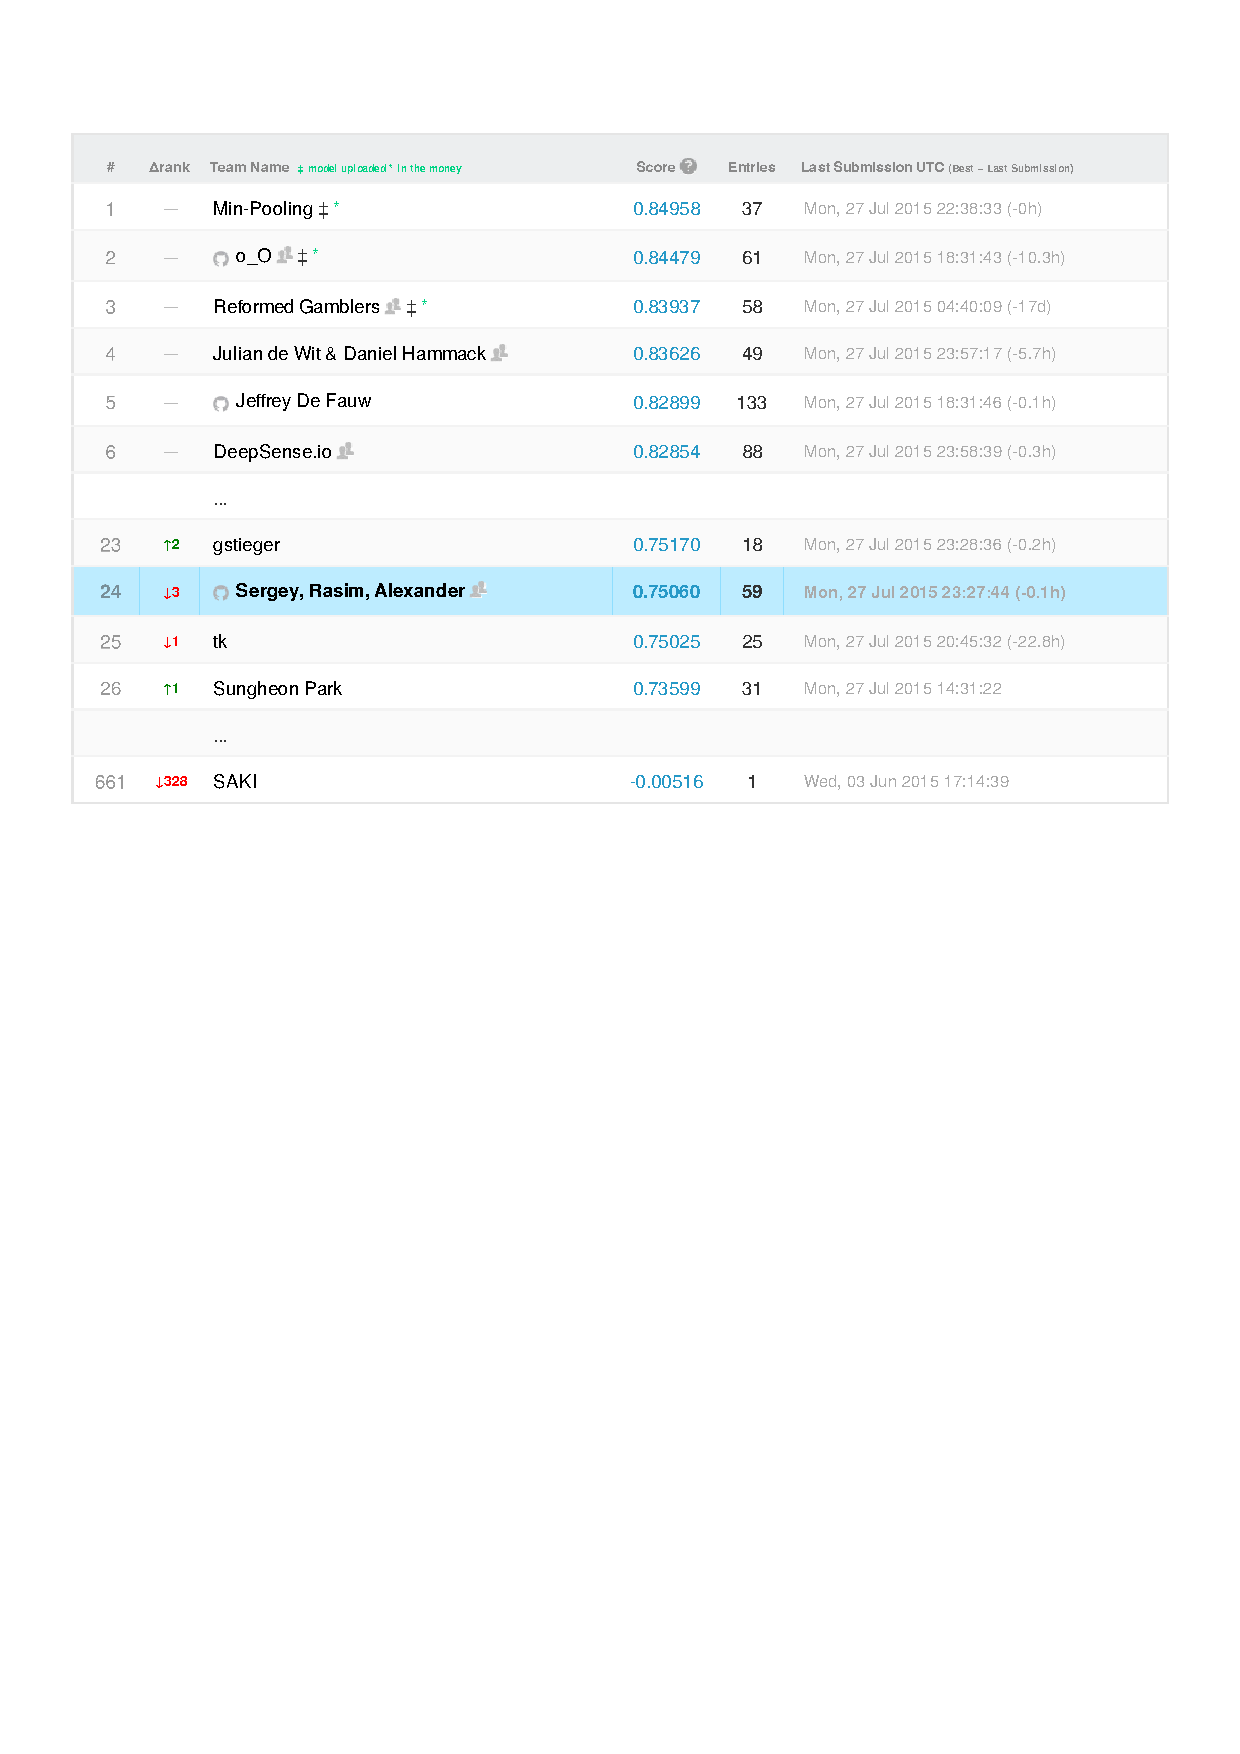
\includegraphics[width=\textwidth]{pics/private_lb_selected.pdf}
\end{figure}
\end{center}
\end{frame}


\begin{frame}\frametitle{Teams distribution on private LB} 
\vspace{-5pt}
\begin{center}
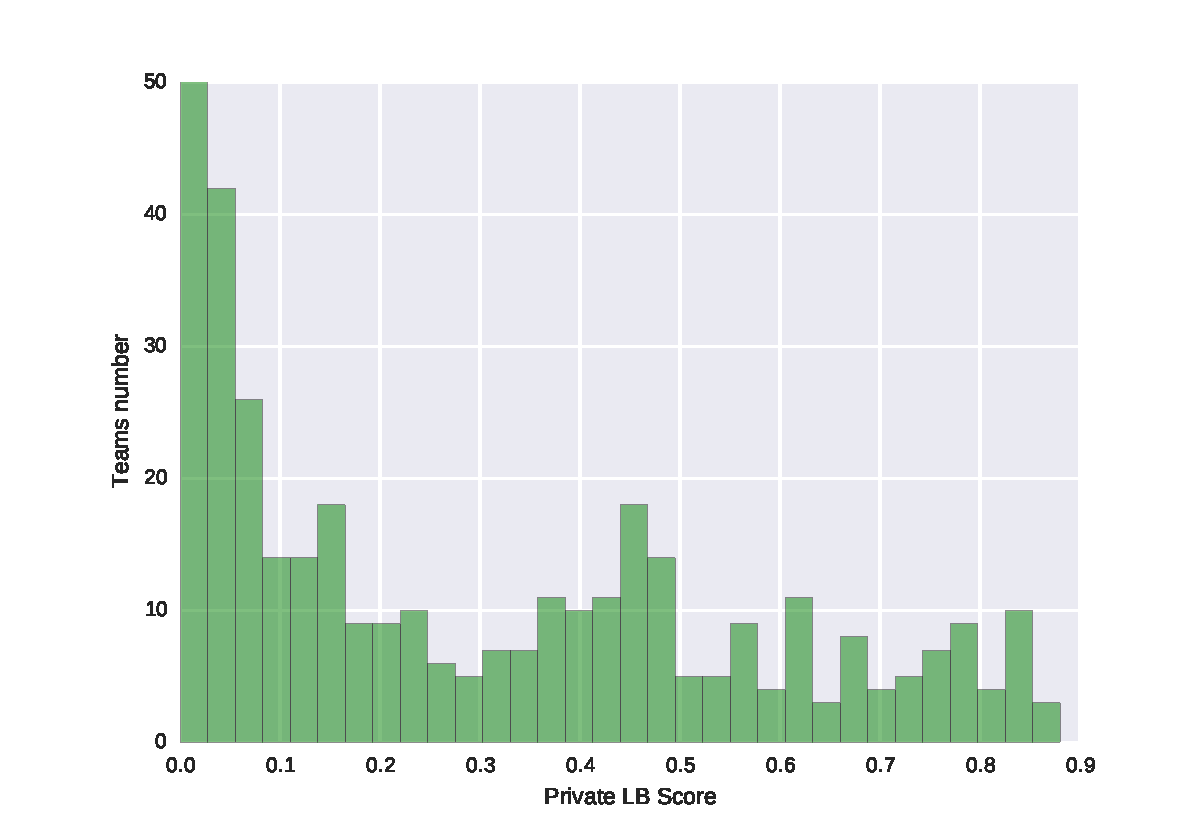
\includegraphics[width=\textwidth]{pics/private_lb_distribution.pdf}
\end{center}
\end{frame}


\begin{frame}\frametitle{} 
\begin{center}
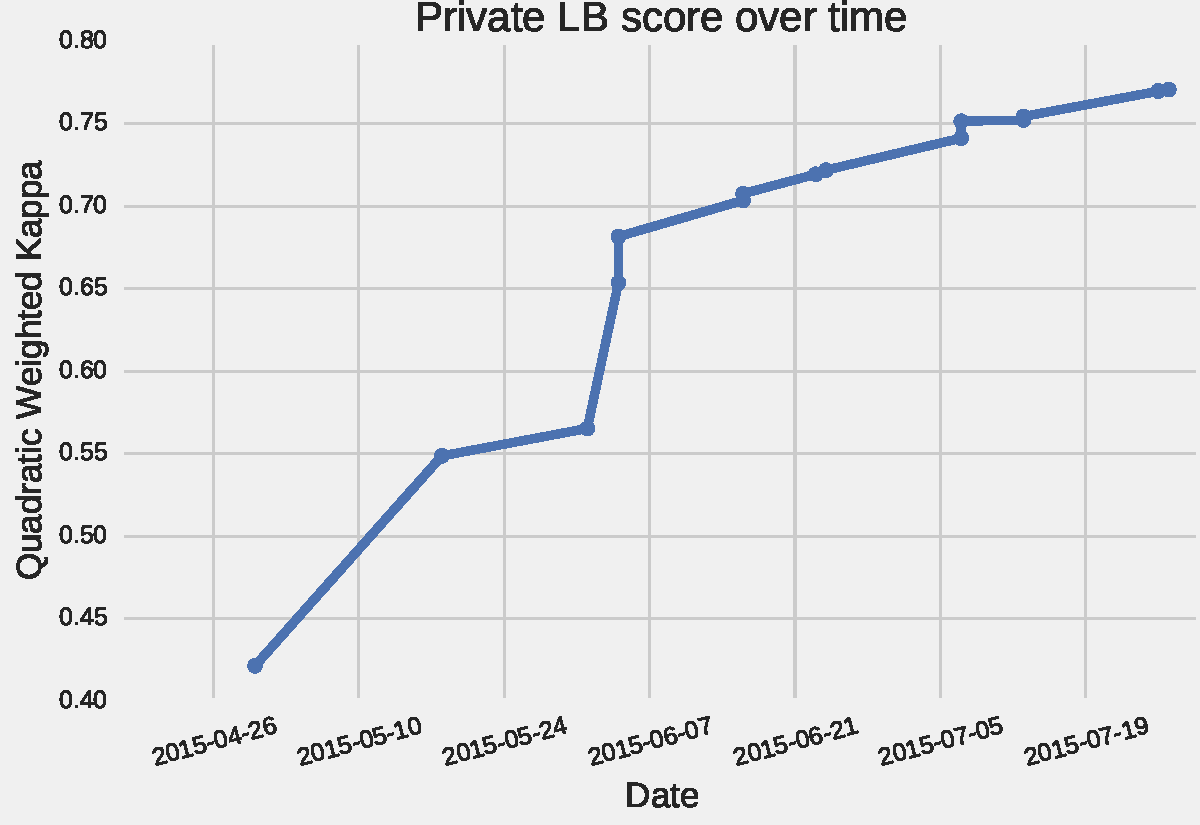
\includegraphics[width=\textwidth]{pics/private_lb_score_increase.pdf}
\end{center}
\end{frame}

%\begin{frame}\frametitle{} 
%\par final leaderboard
%\par + provide leaderboard histogram
%\par + plot score over time
%\end{frame}
